\documentclass[a4paper]{article}
\usepackage[a4paper,includeheadfoot,margin=2.54cm]{geometry}
\usepackage[utf8]{inputenc}
\usepackage[T1]{fontenc}
\usepackage[english]{babel}
\usepackage{graphicx}
\usepackage{float}
\usepackage{pifont}
\usepackage{listings}
\usepackage{hyperref}
\usepackage{xspace}
\usepackage{fancyhdr}
\usepackage{enumitem}
\usepackage{xcolor}
\usepackage{xspace}
\usepackage[export]{adjustbox}
\pagestyle{fancy}
\usepackage{listings}
\usepackage{soul}% http://ctan.org/pkg/soul

\fancyhf{}
\fancyhf[R]{\slshape \rightmark}
\fancyhf[L]{Draft - \today}
\fancyfoot{}
\fancyfoot[C]{\thepage}

\title{Modeling of the ISO 26262 standard}
\author{{D. J. van den Brand}}
\date{\today}

%%%%%%%%%%%%%%%%%%%%%%%%%%%%%%%%%%%%%%%%%%%%%%%%%%%%%%%%%%%%%%%%%%%%
% Custom functions %%%%%%%%%%%%%%%%%%%%%%%%%%%%%%%%%%%%%%%%%%%%%%%%%
%%%%%%%%%%%%%%%%%%%%%%%%%%%%%%%%%%%%%%%%%%%%%%%%%%%%%%%%%%%%%%%%%%%%
\newcommand{\myDef}[2]{\underline{\textsubscript{\textsf{#1}}\hspace{.05cm}#2}}
\newcommand{\isoDef}[1]{\myDef{ISO}{#1}}
\newcommand{\levDef}[1]{\myDef{L}{#1}}
\newcommand{\avizDef}[1]{\myDef{A}{#1}}

\newcommand{\ISO}{ISO 26262 standard\xspace}
\newcommand{\ISOmodel}{ISO 26262 model\xspace}
\newcommand{\ISOFSC}{ISO 26262 Functional safety concept (clause 3.8)\xspace}

\newcommand{\EVL}{EVL\xspace}

% Fix header text
\renewcommand{\sectionmark}[1]{\markright{\thesection\ #1}}
\renewcommand{\subsectionmark}[1]{\markright{\thesubsection\ #1}}
% Set abstract width
\renewenvironment{abstract}
 {\small
  \begin{center}
  \bfseries \abstractname\vspace{-.5em}\vspace{0pt}
  \end{center}
  \list{}{
    \setlength{\leftmargin}{3cm}%
    \setlength{\rightmargin}{3cm}%
  }%
  \item\relax}
 {\endlist}

\begin{document}
\maketitle

\begin{abstract}
This document contains the preliminarily results of a modeling project of the \ISO.
An overview of current literature on modeling of the \ISO is given.
This project aims at generating EVL constraints from the \ISO which can be used to validate automotive projects at an early stage in the design process.
A preliminary set of constraints from the 'Functional safety concept' and 'Specification of software safety requirements' from the \ISO are given.
Also an description of an use case from adaptive cruise control is given to which the validation of constraints is applied.
The actual validation of the use case itself has not yet been done.
\end{abstract}

\section{Introduction} \label{sec:introduction}
In the automotive industry we see that the complexity of the systems is growing rapidly.
Also the control which these systems have over a vehicle is growing besides this.
It's important that these systems remain safe for the users around them.
An important aspect of the safety of the car is functional safety which focuses on assuring safety in the case of a systems failure.
To ensure a system remains safe not only the system itself needs to be analyzed but also the development process.
Especially in the automotive domain where the system development is a multidisciplinary approach.

One of the leading standards from the automotive industry is the \ISO \cite{InternationalOrganizationforStandardization2009}. %\cite{LUNA-36?}
Adhering to such a standard is one of the basic activities to develop safe systems.
However this process can be very time consuming.
Mainly because the standard covers all parts of development, including the early stages.
So when changes are made re-evaluation is often needed. \cite{LUNA-82}.
Next to this an consistent interpretation of such a standard does not exists because domain experts can have different views on the requirements.
Incorporating changes in the \ISO and confirming the validation therefor becomes a difficult task.
Thus an good structure for modeling the \ISO and verifying its compliance at an early stage of development can be of great help.

Earlier work on this has already been done.
Especially for inexperienced readers of the standard is can be really hard to grasp the requirement based format of the \ISO.
System Engineering \cite{Ross2016a} is a book which contains many references to the \ISO and has a good explanation of the basic concepts behind it.
However this book is only meant as background reference and makes no attempt to structurally go through the \ISO.

Also an thesis by Luo was focusing on the \ISO standard \cite{thesis.luna}.
A good framework is proposed on how to model a project according to the \ISO.
Two models are introduced: one which process models the development process and one which models the relevant artifacts which the development process generates.
Also an simple model of the \ISO document itself is proposed which is used in this study.
Also it is concluded that the structural models and process models are applicable in the industry and able to support the development process.

Also Wu et. al. have proposed an formal method to check OCL constraints on safety critical systems in the avionics domain \cite{Wu2015}.
%This is the other end of the story.
Constraints on the design are extracted from the avionics standard.
These are then refined and defined on a model using OCL constraints.
Finally these constraints are then validated against an use case.
This paper has shown that these constraints can be created and effectively applied within an avionics use case.

%
% Scope
%
The goal of this project is to build forward on the previously mentioned two literatures.
And apply the constraints as found by Wu et. al. in the automotive domain.
However the creation of an model for the \ISO is a too big of a task.
%The avionics industry is much more mature in the area of safety compared to the automotive 
To limit the scope of the project an consensus has to be made.
So the model will build forward on a previously generated model at TNO \cite{KhabbazSaberi2017}.
TNO (Netherlands Organization for Applied Scientific Research) is a research company which is closely collaborating with many automotive OEMs and TIER1 suppliers in the world.
The model is still in development and not published but is suffices to give a firm basis.

The remainder of the document some explanation will be given about the \ISO. And the used methodology is explained.
After which the preliminary results are given with preliminary conclusions.

\subsection{Research Question}
The goal of this project will be to find constraints in the \ISO which can be applied early in the development process. So: \textit{What are the highest level of constraints one can extract from the \ISO which are still effective?}\\
Next to this question it would be nice to validate this with the help of a use case so there will also be a Use Case on adaptive cruise control to validate these constraints and look for false positives and false negatives with respect to the extend to which the constraint adherence process represents the \ISO compliance.

\subsection{\ISO}
The \ISO document is divided up into 10 parts. Each part roughly contains text which describes how to use the document and a list of requirements. Except for part 1 and 10 (respectively named definitions and guidelines) which only provide additional information which is only used in the other parts.
Each part consists of a number of clauses which group certain requirements together by topic.
The notation of 3-8 will be used denoting clause eight of the third part of the \ISO.
Each clause needs a certain input which can come from external sources or other clauses.
And it produces a certain output in form of a project artifact which are called work documents. These work documents are always an results of some specified requirements.
Next to this each clause has a set of requirements which will denote: a certain process which has to be completed or a certain constraint which the system should adhere to.
Sometimes these requirements are statements which need to be adhered to and other are mere recommendations.
The requirements are labeled with an id, e.g. 8.4.2.4, corresponding to the section of the document. Where the first number of the id denotes the corresponding clause.
Also in addition requirements can have extra sections attached to them with additional notes or examples.

\begin{figure}[h]
\centering
\includegraphics[width=.65\textwidth]{iso_model_simplified.png}
\caption{\ISO model}
\label{fig:iso_model_simplified}
\end{figure}

\subsection{Scope}
The project will focus on the modeling of the 'Functional safety concept' (clause 3-8).
The inputs for this clause consist of:
\begin{itemize}
\item Item definition (work product of clause 3-5)
\item Hazard analysis and risk assessment (work product of clause 3-7)
\item Preliminary architectural assumptions (external)
\item Functional concept (external)
\item Operating modes and system states (external)
\end{itemize}
Next to this it also directly relies on:
\begin{itemize}
\item Specification of software safety requirements (clause 8-6)
\item Requirements decomposition with respect to ASIL tailoring (clause 9-5)
\item Analysis of dependent failures (clause 9-7)
\end{itemize}
The inputs are available from the model form TNO but clause 8-6 really imposed an missing link to generating the constraints so the final scope is set on the two clauses 8-6 and 3-8. Because clause 8-6 did not have any dependencies.

\section{Methodology} \label{sec:methodology}
A high level overview of the modeling process is denoted in Figure \ref{fig:ISO-modeling-methodology}.
The first action which is performed is to extract a clause in textual form from the \ISO.
This is done in a fairly straight forward manner for every part.

After this two models are extracted, following the same methodology from Luo \cite{thesis.luna}.
The project model defines the structure of the data and artifacts of the development process.
The process model will be present in the interpretation file, or will later be added.
the second model contains the interpretation of the \ISO.
This model contains all the design decisions which were made during the interpretation.
A more detailed version of this can be seen in Section \ref{sec:interpretation}.
Continuously the project model and interpretation model are used as input to generate and validation model.
This is a single EVL file for every clause.
This contains all the constraints and is coupled to the original text of the \ISO.
This model is also directly executable to be used against a actual project instance by means of a use case.

\begin{figure}[ht]
\centering
\includegraphics[width=.7\textwidth]{ISO-modeling-methodology.png}
\caption{Methodology}
\label{fig:ISO-modeling-methodology}
\end{figure}

\subsection{Interpretation proccess} \label{sec:interpretation}
the interpretation process is executed by first classifying the requirements.
This way the biggest part of the structure can be created first.
There are four classifications of the requirements which have been found:
\begin{description}
\item[informal] These requirements are not really concise. They usually only introduce an concept without making hard claims about the properties.
\item[structure] These requirements denote which attributes or relations certain elements should have. Next to the existence of attributes also the simple cardinality constraints on the attributes are captured here. Mainly because the cardinality is almost always denoted when an new concept is introduced.
% The structural requirements are usally not written down in an explicit manner. They also show up almost everywhere.
\item[constraint] These requirements denote an actual constraint which needs to be adhered to. So this will not only denote something about the simple existence of a relation but also depends on the information contained of in the elements.
\end{description}

After the requirements are classifies the structural requirements are evaluated first with respect to the project model.
For each concept and relationship that is encountered it is added to the model.
This way the model will become to big to comprehend or work with but this is not needed.
It's only needed to find a mapping from the project instance to this bigger model and the original project instance will be corrected, not the mapped model.
After this the remaining requirements are interpreted with respect to constraints.
In more detail the following elements are captured for each requirement:
\begin{description}
%\item[id] An unique identifier
\item[model elements] For traceability every element which is created in the project model is linked to an interpretation of the requirement. This is mainly used to keep the model and interpretation tightly coupled during the design process.
\item[classification] The classifications the requirements belong to, as explained above.
\item[constraints] An specification for the \EVL which is corresponds to this requirement. These are classified as shown in Section \ref{sec:Constraint classification}
\item[status] To keep track of the validation of the interpretation.
\end{description}

\subsubsection{Constraint classification} \label{sec:Constraint classification}
Each requirements gets one or more labels from the classifications explained below:
\begin{description}
\item[structural]
The vast majority of the requirements say something about the existence of certain development artifacts.
These will be labeled as structural constraints.
Next to this an design decision should occasionally be made on the modeling of the structural model.
These could give rise to additional constraints not explicitly present in the \ISO but for the creation of an more comprehensible model.
Although these are avoided as much as possible some extra constraints are needed to ensure a valid project model.
Also next to the possible existence of some artifact there is often also a cardinality constraint implicitly denoted.
These are not included in the validation process an will thus not be labeled.
For example: "An requirement should have a unique identifier" could better be captured using "\texttt{unique attr String[1] id}" as opposed to an separate constraint.
They are to be captured in the project model itself as this would otherwise flood the validation with many trivial constraints.
Because the traceability is kept for each model element it can always easily be looked up where such a cardinality constraint comes from if it failes and is not trivial.

\item[$++$, $+$ and $\circ$]
Sometimes the \ISO has a table which already denote a classification of the requirements.
the constraints that follow from these tables are copied from the \ISO and denote: Highly recommended, recommended and no recommendation respectively.

\item[required]
Certain requirements say something about the relation between artifacts or have more complicated cardinality constraints.
These constraints have to be satisfied on the project in order to adhere to the \ISO.

\item[check]
Other constraints are related to an process which has to be performed.
This is best explained by example:
All safety requirements need to be unambiguous.
This is modeled by means of a simple boolean field on the safety requirements class which should be set to true when the check has been completed.
A constraint for this then thus becomes that the unambiguous check should have been done.

\item[other] %implicit
And finally some requirements are not clearly specified or impose some rather trivial constraints that have to be met.
\end{description}


\subsection{Epsilon Validation Language (EVL)}
Instead of OCL constraints on UML models EVL is used on Ecore models from the Epsilon framework of Eclipse.
This language has additional support for feedback on the validation failures.
Because every failure will always correspond to an specific requirement from the \ISO its sensible to show this to the user on failure.
In addition a severity level could be added to an EVL constraint to give requirements a priority similar to the \ISO: needed and recommended requirements. \cite{Kolovos2009}
Also Emfatic files provide a easy to write specification language for the Ecore models which in turn has an visually appealing representation format already freely available with Eclipse \footnote{https://www.eclipse.org/epsilon/}.


\section{Preliminairy result} \label{sec:result}
In this section the findings of the above methodology are presented.
A total of 33 requirements have been interpreted, resulting on 28 constraints, as seen in Table \ref{tbl:constraint-count}.

\begin{table}[]
%		safety requirements	functional safety concept
%requirement classification	structure_intro	2	2
%	clause_input	1	1
%	structure	10	4
%	ocl	12	3
%	total	22	11
%constraints	check	8	0
%	++	2	0
%	+	3	0
%	fixes	1	0
%	satisfies	6	6
%	warning	0	1
%	total	20	7
\centering
\begin{tabular}{ll|l|l|}
\cline{3-4}
                                                 &                  & safety requirements & functional safety concept \\ \hline
\multicolumn{1}{|l|}{requirement classification} & structure\_intro & 2                   & 2                         \\ \cline{2-4} 
\multicolumn{1}{|l|}{}                           & clause\_input    & 1                   & 1                         \\ \cline{2-4} 
\multicolumn{1}{|l|}{}                           & structure        & 10                  & 4                         \\ \cline{2-4} 
\multicolumn{1}{|l|}{}                           & ocl              & 12                  & 3                         \\ \cline{2-4} 
\multicolumn{1}{|l|}{}                           & total            & 22                  & 11                        \\ \hline
\multicolumn{1}{|l|}{constraint classification}                & check            & 8                   & 0                         \\ \cline{2-4} 
\multicolumn{1}{|l|}{}                           & ++               & 2                   & 0                         \\ \cline{2-4} 
\multicolumn{1}{|l|}{}                           & +                & 3                   & 0                         \\ \cline{2-4} 
\multicolumn{1}{|l|}{}                           & fixes            & 1                   & 0                         \\ \cline{2-4} 
\multicolumn{1}{|l|}{}                           & satisfies        & 6                   & 6                         \\ \cline{2-4} 
\multicolumn{1}{|l|}{}                           & warning          & 0                   & 1                         \\ \cline{2-4} 
\multicolumn{1}{|l|}{}                           & total            & 20                  & 8                         \\ \hline
\end{tabular}
\caption{Number classifications and constraints} \label{tbl:constraint-count}
\end{table}

Below one of the more interesting requirements are denoted.
As a reference the requirements itself are also provided in the appendix.
\begin{itemize}
\item[3-8.4.2.2] At least one functional safety requirement shall be specified for each safety goal
\item[3-8.4.2.4] All state transitions to and from a safe state need to have a condition
\item[8-6.4.1.1] All safety requirements with ASIL A or B are recommended to have an informal notation style
\item[8-6.4.2.4.a] All safety requirements should be unambiguous
\item[8-6.4.3.2] Safety requirements should be traceable to either an lower requirement in the hierarchy or an element in the design.
\end{itemize}

\section{Use case overview}
In addition an use case is presented which will be validated against the constraints.
This use case consists of an Adaptive Cruise Control (ACC) software system.
In collaboration with TNO the following clauses are being applied in the development of this item:
\begin{itemize}
\item 3-5 Item definition. In order to create a functional safety concept the item should be defined. (sufficient)
\item 3-6 Safety lifecycle. This is skipped because the use case does not build upon previous elements.
\item 3-7.5.1 Hazard Analysis and Risk assessment (being reviewed)
\item 3-7.5.2 Safety goals (being reviewed)
\item 3-8.5.1 Functional safety concept (work in progress)
\end{itemize}

In Figure \ref{fig:ACC system overview} an overview is shown of the relation of the item to other items in the vehicle.
Note that this diagram is based on the AUTOSAR methodology and does not include a deployment scheme on how these software component will eventually be mapped on the hardware \cite{Briciu2013}.
The use case concerns the package at the bottom, named \textit{ACC}.
It communicated to all other component in the system (and to the other component) via either van CAN interface from the communications package or via shared memory on the same controller.
Also note that the ObstacleDetector system is considered to be separate as this will be considered as an external technology which will not be part of the \textit{ACC} item.

The two presented components are shown in more detail below.
In Figure \ref{fig:ACC Control component} the flow diagram of the \textit{ACC Control} component is shown.
Here it can be seen which messages it should receive and send to the other component in the vehicle.
An fixed simulation time is chosen which send the appropriate control messages to the throttle and break based on the latest known distance estimation to vehicles in front and motion of the car.

The flow diagram of the second component is shown in Figure \ref{fig:ACC Buttons}.
This component manages the input from the user on the steering wheel to configure the system.
It relays state changes directly to the network and sends configuration changes regarding the desired speed and distance to the vehicle in front.

\begin{figure}[h!]\centering
	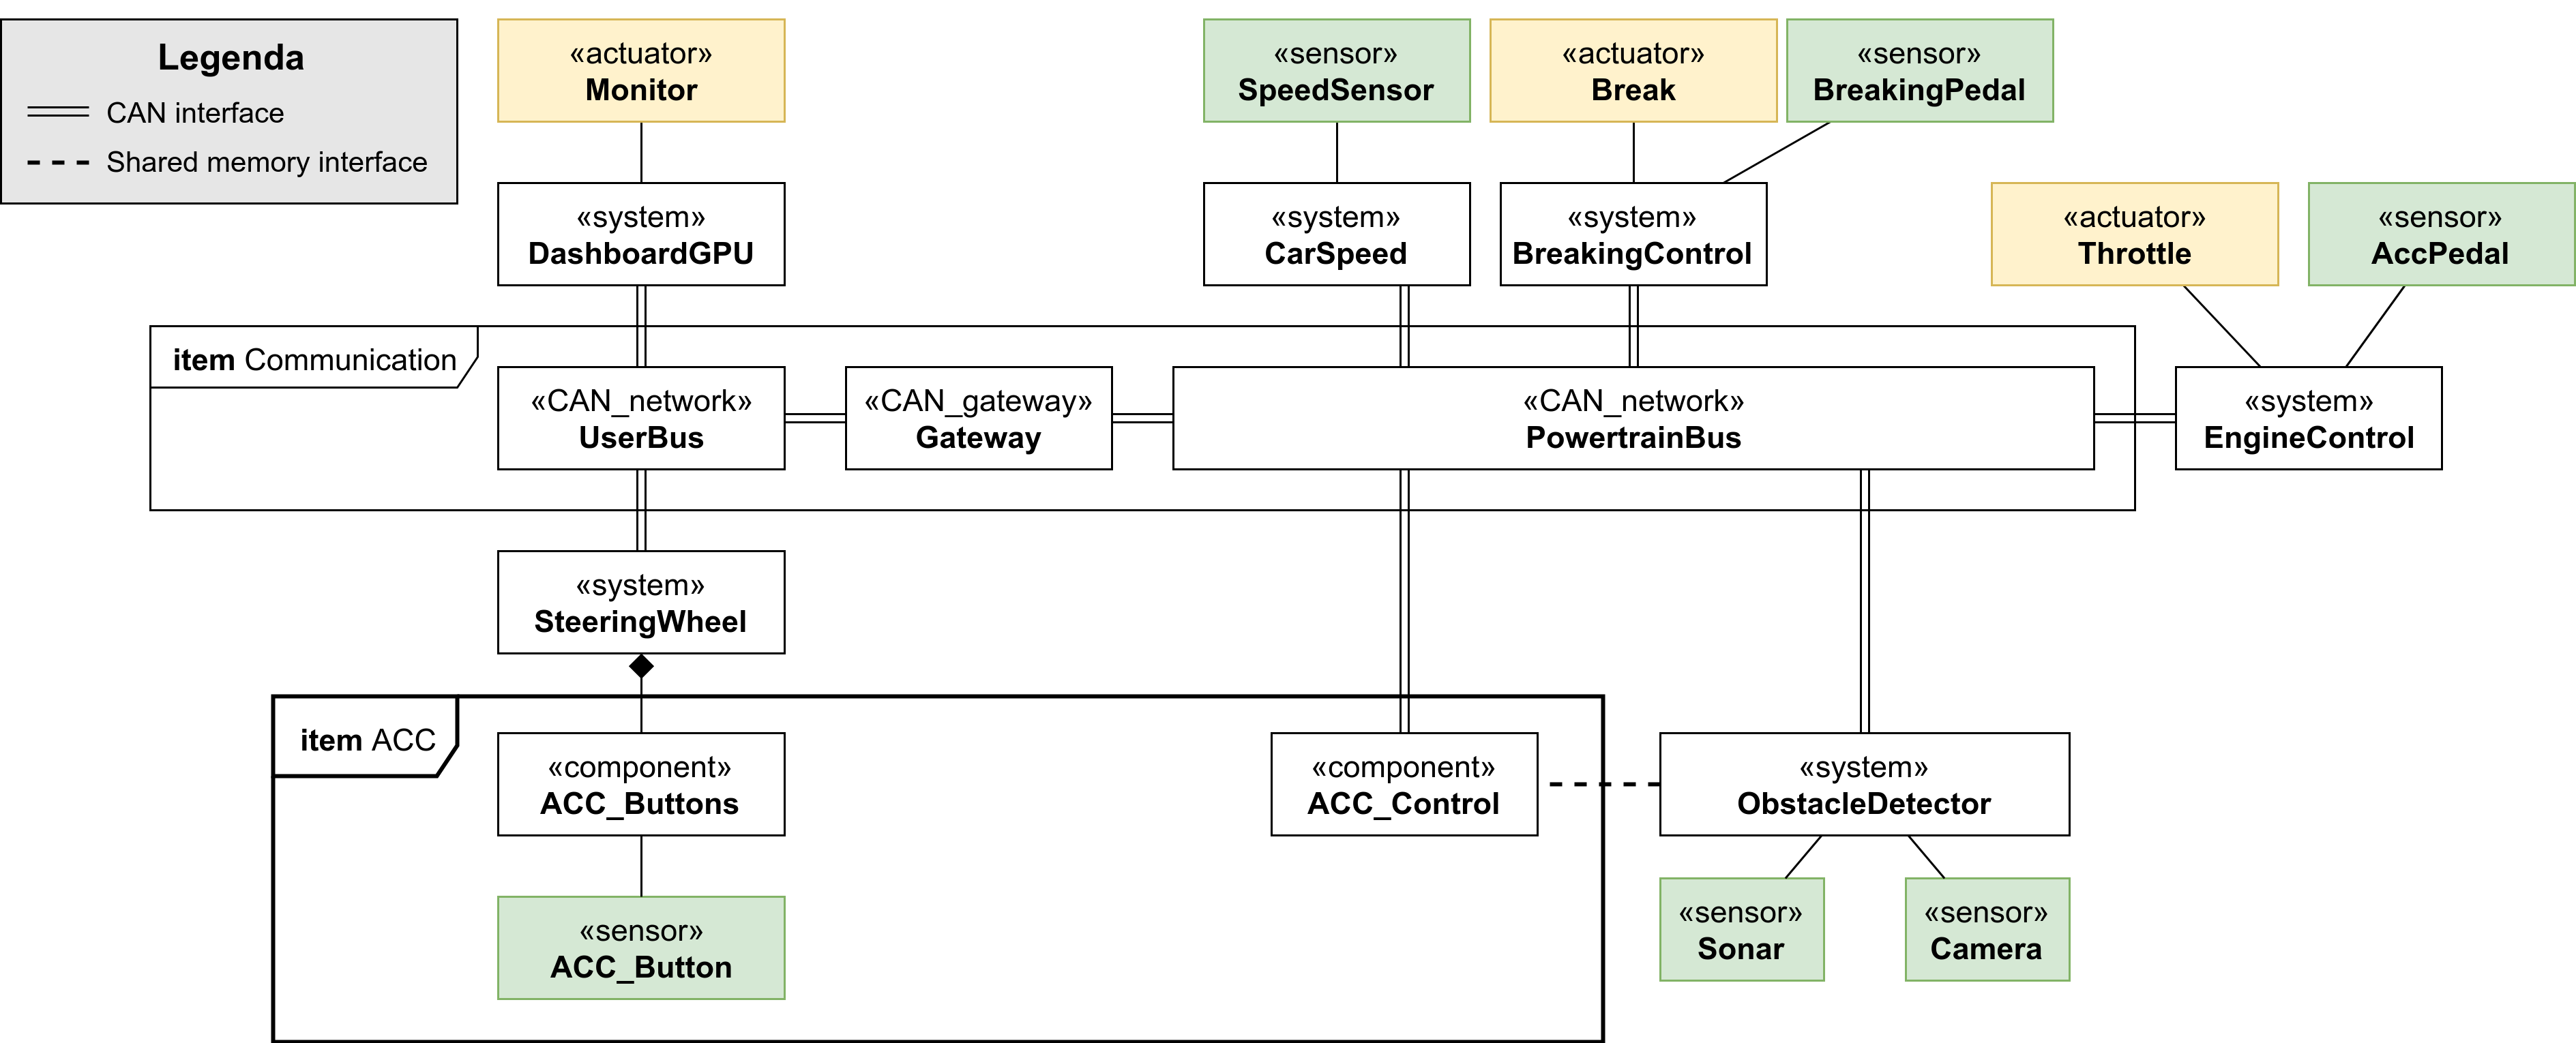
\includegraphics[width=\textwidth]{ACC_system_overview.png}
	\caption{\textit{ACC} item depencies overview}  \label{fig:ACC system overview}
\end{figure}
\begin{figure}[h!]\centering
	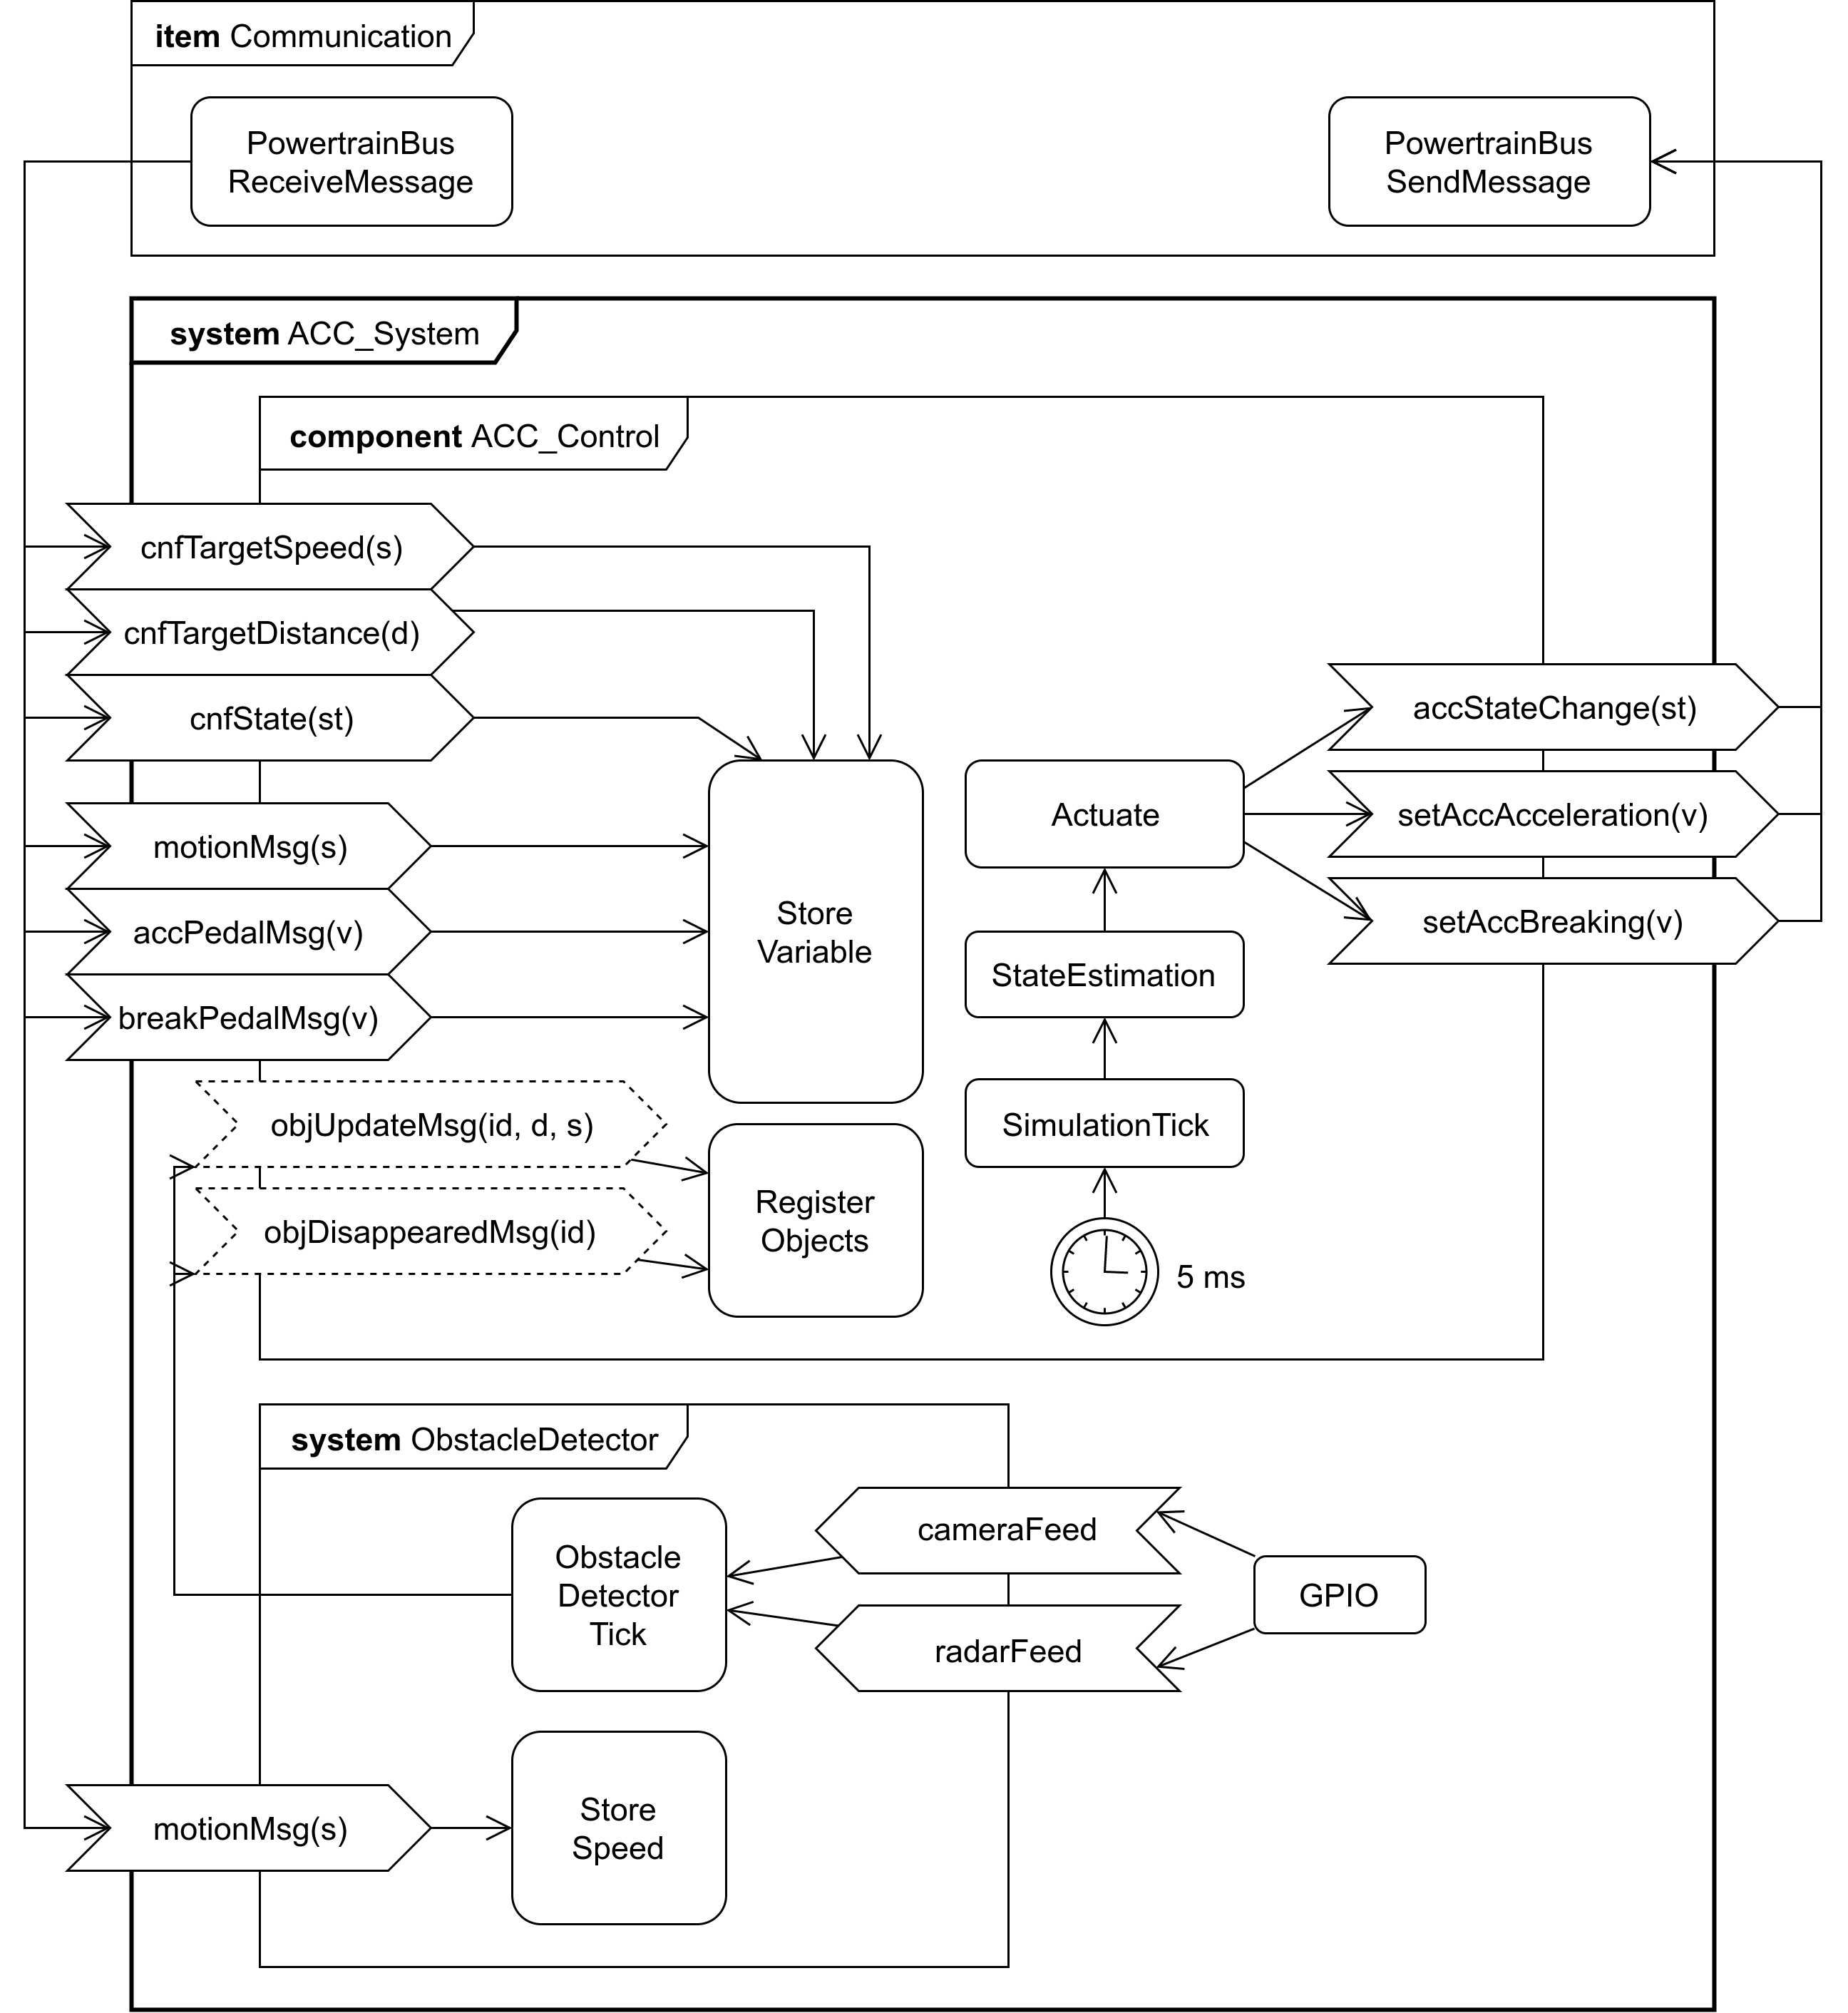
\includegraphics[width=\textwidth]{ACC_Control_functions.png}
	\caption{\textit{ACC Control} component preliminairy architectural assumptions}  \label{fig:ACC Control component}
\end{figure}
\begin{figure}[h!]\centering
	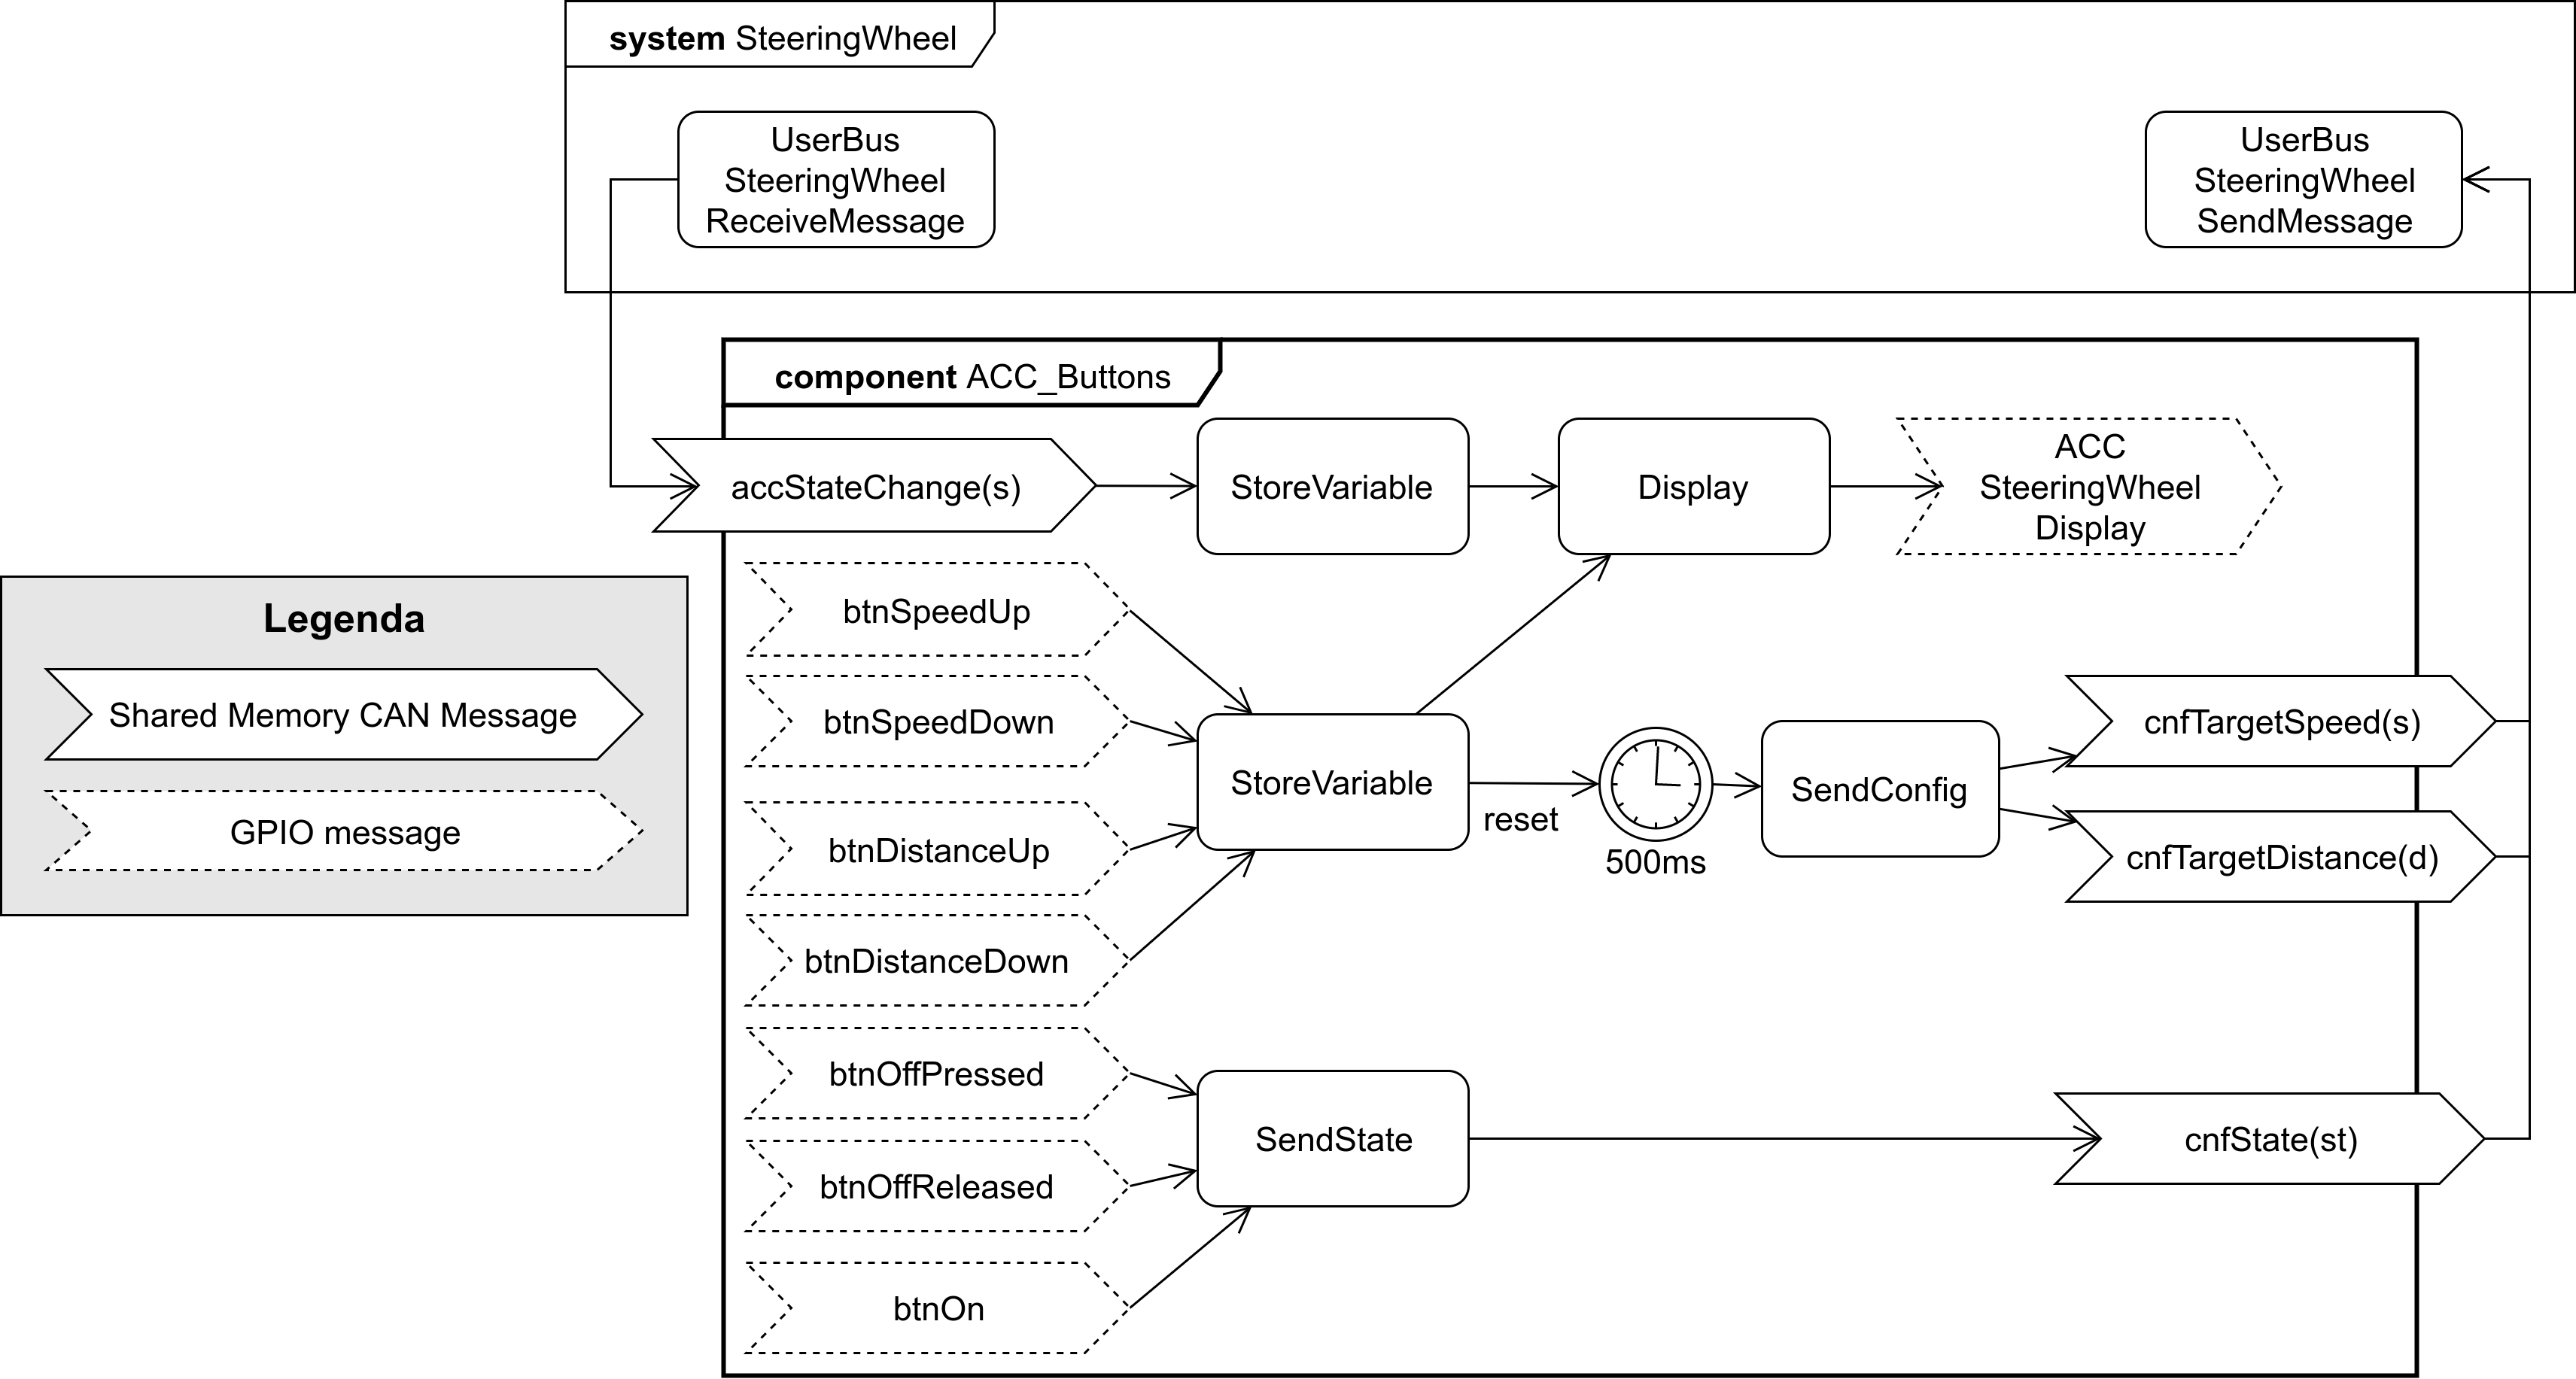
\includegraphics[width=0.85\textwidth]{ACC_Buttons_functions.png}
	\caption{\textit{ACC Buttons} component preliminairy architectural assumptions}  \label{fig:ACC Buttons}
\end{figure}

\section{Preliminairy conclusion} \label{sec:conclusion}
The modeling process takes a lot more time then expected.
The generation of the use case is also a slow process.
But steady the project is gaining more momentum.
This methodology is presenting some constraints which are a good representation for the \ISO and if the supporting processes are executed correctly I expect them to be equivalent to the \ISO clause itself.
However this still needs to be verified by TNO.

The use case will probably not give many violations of the constraints which are presented.
However it greatly helps in understanding the \ISO and figuring out where the constraints could be applied.


\bibliographystyle{plain}
\bibliography{bib.bib}{}

% Gohst section
%\refstepcounter{section}%
%\addcontentsline{toc}{section}{\protect\numberline{\thesection}Appendix}%


\newpage
\renewcommand{\thesection}{}
\sectionmark{Appendix}
\begin{figure}[h!]\centering
	\makebox[\textwidth]{\includegraphics[trim={1cm 14cm 0 1cm},clip,width=0.9\paperwidth]{fsc_project_model.pdf}}
	\caption{\textit{Functional safety concept} project model}  \label{fig:Functional safety concept project model}
\end{figure}
\section*{Constraints of clause 3-8}
Figure \ref{fig:Functional safety concept project model} contains the model of the Functional Safety Concept. And below the corresponding EVL constraints are listed.

\lstset{language=OCL, morekeywords={constraint, check, message, guard, fix, title, do}}%, basicstyle=\ttfamily}
\begin{lstlisting}
context FunctionalSafetyRequirement {
 constraint satisfies_c3_r8_4_2_1 {
  check : self.derrived_from_sg.length() > 0
          or self.derrived_from_ss.length() > 0
  message : "3-8.4.2.1 satisfies 0: ISO requirement: The functional safety requirements shall be derived from the safety goals and safe states, considering the preliminary architectural assumptions, functional concept, operating modes and system states."
 }
}
context SafetyGoal {
 constraint satisfies_c3_r8_4_2_2 {
  check : FunctionalSafetyRequirement.all().exists(
          fsr | fsr.derrived_from_sg.includes(self))
  message : "3-8.4.2.2 satisfies 0: ISO requirement: At least one functional safety requirement shall be specified for each safety goal."
 }
}
context TechnicalStateTransition {
 guard : SafeState.all().exists(s | s.transition_to.includes(self)
         or s.transition_from.includes(self))
 constraint satisfies_c3_r8_4_2_4 {
  check : self.do_condition.length() > 0
          and self.rev_condition.length() > 0
  message : "3-8.4.2.4 satisfies 0: All state transitions for SafeState need to have a condition"
 }
}
context SafeState {
 constraint satisfies_c3_r8_4_2_5 {
  check : (not self.transition_to.exists(t | t.isKindOf(SwitchOffTransition)
           and t.duration.isDefined() and t.duration.direct))
          implies self.emergency_operation.length() > 0
  message : "3-8.4.2.5 satisfies 0: ISO requirement: If a safe state cannot be reached by immediately switching off, an emergency operation shall be specified."
 }
}
context Actor {
 constraint satisfies_c3_r8_4_2_6_b__n0 {
  check : Actor.means.length() > 0
  message : "3-8.4.2.6.b satisfies 0: ISO requirement: If assumptions are made on the necessary actions of the driver, or other endangered persons, in order to comply with the safety goals:The adequate means and controls of the driver or other endangered persons shall be specified in the functional safety concept; "
 }
 constraint satisfies_c3_r8_4_2_6_b__n1 {
  check : Actor.controls.length() > 0
  message : "3-8.4.2.6.b satisfies 1: ISO requirement: If assumptions are made on the necessary actions of the driver, or other endangered persons, in order to comply with the safety goals:The adequate means and controls of the driver or other endangered persons shall be specified in the functional safety concept; "
 }
}

\end{lstlisting}
\newpage
\begin{figure}[h!]\centering
	\makebox[\textwidth]{\includegraphics[trim={1cm 8cm 1cm 1cm},clip,width=0.9\paperwidth]{javaprint4703700183606300293.pdf}}
	\caption{\textit{Safety requirements} project model} \label{fig:Safety requirements project model}
\end{figure}
\section*{Constraints of clause 8-6}
Figure \ref{fig:Safety requirements project model} contains the model of the Safety requirements project model. And below the corresponding EVL constraints are listed.

\begin{lstlisting}
context SafetyRequirement {
   constraint p_c8_r6_4_1_1_n0 {
      guard : /* self.asil IS_ASIL_C_OR_D */
      check : self.notation=RequirementNotationStyle.informal
      message : "8-6.4.1.1 + 0: ISO requirement: To achieve the characteristics of safety requirements listed in 6.4.2.4, safety requirements shall be specified by an appropriate combination of"
   }
   constraint p_c8_r6_4_1_1_n1 {
      guard : /* self.asil IS_ASIL_A_OR_B */
      check : self.notation=RequirementNotationStyle.semi_formal
      message : "8-6.4.1.1 + 1: ISO requirement: To achieve the characteristics of safety requirements listed in 6.4.2.4, safety requirements shall be specified by an appropriate combination of"
   }
   constraint p_c8_r6_4_1_1_n2 {
      guard : /* self.asil IS_ASIL_A_OR_B_OR_C_OR_D */
      check : self.notation=RequirementNotationStyle.formal
      message : "8-6.4.1.1 + 2: ISO requirement: To achieve the characteristics of safety requirements listed in 6.4.2.4, safety requirements shall be specified by an appropriate combination of"
   }
}

context SafetyRequirement {
   constraint pp_c8_r6_4_1_1_n0 {
      guard : /* self.asil IS_ASIL_A_OR_B */
      check : self.notation=RequirementNotationStyle.informal
      message : "8-6.4.1.1 ++ 0: ISO requirement: To achieve the characteristics of safety requirements listed in 6.4.2.4, safety requirements shall be specified by an appropriate combination of"
   }
   constraint pp_c8_r6_4_1_1_n1 {
      guard : /* self.asil IS_ASIL_C_OR_D */
      check : self.notation=RequirementNotationStyle.semi_formal
      message : "8-6.4.1.1 ++ 1: ISO requirement: To achieve the characteristics of safety requirements listed in 6.4.2.4, safety requirements shall be specified by an appropriate combination of"
   }
}

context SafetyRequirement {
   constraint satisfies_c8_r6_4_2_2 {
      check : self.derrived_from.forAll(p|p.asil = self.asil)
      message : "8-6.4.2.2 satisfies 0: ISO requirement: Safety requirements shall inherit the ASIL from the safety requirements from which they are derived."
      fix {
         title : "Set the asil to the same as a random parent"
         do {
            self.asil=self.parent.random().asil;
         }
      }
   }
}
context SafetyRequirement {
   constraint satisfies_c8_r6_4_2_3 {
      check : self.allocated_to_element.isDefined() or self.allocated_to_item.isDefined()
      message : "8-6.4.2.3 satisfies 0: ISO requirement: Safety requirements shall be allocated to an item or an element."
   }
}
pre SafetyRequirement {
   // CREATE CHECK unambiguous
   for (x : SafetyRequirement in SafetyRequirement.all().select(x|x.unambiguous.isUndefined()) ) { x.unambiguous = new Check(); }for (x : SafetyRequirement in SafetyRequirement.all()) { x.unambiguous.description = "Safety requirements shall have the following characteristics:unambiguous and comprehensible; "; }
   // CREATE CHECK comprehensible
   for (x : SafetyRequirement in SafetyRequirement.all().select(x|x.comprehensible.isUndefined()) ) { x.comprehensible = new Check(); }for (x : SafetyRequirement in SafetyRequirement.all()) { x.comprehensible.description = "Safety requirements shall have the following characteristics:unambiguous and comprehensible; "; }
}
context SafetyRequirement {
   constraint satisfies_c8_r6_4_2_4_a_n0 {
      check : self.unambiguous.validated
      message : "8-6.4.2.4.a satisfies 0: ISO requirement: Safety requirements shall have the following characteristics:unambiguous and comprehensible; "
   }
   constraint satisfies_c8_r6_4_2_4_a_n1 {
      check : self.comprehensible.validated
      message : "8-6.4.2.4.a satisfies 1: ISO requirement: Safety requirements shall have the following characteristics:unambiguous and comprehensible; "
   }
}
pre SafetyRequirement_1 {
   // CREATE CHECK atomic
   for (x : SafetyRequirement in SafetyRequirement.all().select(x|x.atomic.isUndefined()) ) { x.atomic = new Check(); }for (x : SafetyRequirement in SafetyRequirement.all()) { x.atomic.description = "Safety requirements shall have the following characteristics:atomic; "; }
}
context SafetyRequirement {
   constraint satisfies_c8_r6_4_2_4_b {
      check : self.atomic.validated
      message : "8-6.4.2.4.b satisfies 0: ISO requirement: Safety requirements shall have the following characteristics:atomic; "
   }
}
pre SafetyRequirement_1 {
   // CREATE CHECK internally_consistent
   for (x : SafetyRequirement in SafetyRequirement.all().select(x|x.internally_consistent.isUndefined()) ) { x.internally_consistent = new Check(); }for (x : SafetyRequirement in SafetyRequirement.all()) { x.internally_consistent.description = "Safety requirements shall have the following characteristics:internally consistent; "; }
}
context SafetyRequirement {
   constraint satisfies_c8_r6_4_2_4_c {
      check : self.internally_consistent.validated
      message : "8-6.4.2.4.c satisfies 0: ISO requirement: Safety requirements shall have the following characteristics:internally consistent; "
   }
}
pre SafetyRequirement_1 {
   // CREATE CHECK feasible
   for (x : SafetyRequirement in SafetyRequirement.all().select(x|x.feasible.isUndefined()) ) { x.feasible = new Check(); }for (x : SafetyRequirement in SafetyRequirement.all()) { x.feasible.description = "Safety requirements shall have the following characteristics:feasible; and "; }
}
context SafetyRequirement {
   constraint satisfies_c8_r6_4_2_4_d {
      check : self.feasible.validated
      message : "8-6.4.2.4.d satisfies 0: ISO requirement: Safety requirements shall have the following characteristics:feasible; and "
   }
}
pre SafetyRequirement_1 {
   // CREATE CHECK verifiable
   for (x : SafetyRequirement in SafetyRequirement.all().select(x|x.verifiable.isUndefined()) ) { x.verifiable = new Check(); }for (x : SafetyRequirement in SafetyRequirement.all()) { x.verifiable.description = "Safety requirements shall have the following characteristics:verifiable. "; }
}
context SafetyRequirement {
   constraint satisfies_c8_r6_4_2_4_e {
      check : self.verifiable.validated
      message : "8-6.4.2.4.e satisfies 0: ISO requirement: Safety requirements shall have the following characteristics:verifiable. "
   }
}
context SafetyRequirement {
   constraint SR_level_respects_hierachy {
      check : self.derrived_from.forAll(
              parent | parent.level >= self.level)
      message : "8-6.4.3.1.a SR_level_respects_hierachy: Derrive relation should respect the structural hierarchy"
   }
}
context RequirementGroup {
   constraint satisfies_c8_r6_4_3_1_b {
      check {
         var rqs = SafetyRequirement.all().select(sr|sr.group=self);
         if(rqs.isEmpty()){return true;}
         var group_level = rqs.random().level;
         return rqs.forAll(sr|sr.level=group_level);
      }
      message : "8-6.4.3.1.b satisfies 0: ISO requirement: The collection of safety requirements shall have the following properties:organizational structure according to an appropriate grouping scheme;"
   }
}
pre RequirementLevel {
   // CREATE CHECK all_reqs_cover_parent
   for (x : RequirementLevel in RequirementLevel.all().select(x|x.all_reqs_cover_parent.isUndefined()) ) { x.all_reqs_cover_parent = new Check(); }for (x : RequirementLevel in RequirementLevel.all()) { x.all_reqs_cover_parent.description = "The collection of safety requirements shall have the following properties:completeness;"; }
}
context RequirementLevel {
   guard : self.value < RequirementLevel.all().select(e|e.name="SG").random().value
   constraint satisfies_c8_r6_4_3_1_c {
      check : self.all_reqs_cover_parent.validated
      message : "8-6.4.3.1.c satisfies 0: ISO requirement: The collection of safety requirements shall have the following properties:completeness;"
   }
}
pre SafetyRequirement_1 {
   // CREATE CHECK contradicts_another
   for (x : SafetyRequirement in SafetyRequirement.all().select(x|x.contradicts_another.isUndefined()) ) { x.contradicts_another = new Check(); }for (x : SafetyRequirement in SafetyRequirement.all()) { x.contradicts_another.description = "The collection of safety requirements shall have the following properties:external consistency;"; }
}
context SafetyRequirement {
   constraint satisfies_c8_r6_4_3_1_d {
      check : self.contradicts_another.validated
      message : "8-6.4.3.1.d satisfies 0: ISO requirement: The collection of safety requirements shall have the following properties:external consistency;"
   }
}
context SafetyRequirement {
   constraint SR_in_hierachy {
      guard : self.level < RequirementLevel.all().get(e|e.name="SG"))
      check : not self.derrived_from.isEmpty()
      message : "8-6.4.3.2 SR_in_hierachy: ISO requirement: Safety requirements shall be traceable with reference being made to:"
   }
   constraint SR_covers_elements {
      guard : not SafetyRequirement.all().exists(
              sr|sr.derrived_from.contains(self)) // Only lowest requirements
      check : self.allocated_to_element.isDefined()
      message : "8-6.4.3.2 SR_covers_elements: ISO requirement: Safety requirements shall be traceable with reference being made to:"
   }
}
\end{lstlisting}

\end{document}
